\documentclass[12pt, letter]{article}
\usepackage[letterpaper, margin=1in]{geometry}
\usepackage{setspace}
\usepackage{amsmath}
\usepackage{graphicx}
\usepackage{hyperref}
\usepackage{indentfirst}
\usepackage{subcaption}

\title{Multi-Agent Reinforcement Learning\\
	\large{ Course Project Proposal}}
	\author{
		Denis Osipychev\thanks{deniso2@illinois.edu} \\
		Yizhi Fang\thanks{yfang10@illinois.edu} \\
	}
	\date{}
	
\begin{document}
\singlespacing
		
\maketitle
\newpage
		
		
\section{Introduction}
The recent advantages of Reinforcement Learning (RL) algorithms already demonstrated the ability of RL agents learn and perform many complex tasks previously attained by a human only. Agents involving deep RL have been successfully applied to many challenging problems from playing a range of Atari 2600 video games at a superhuman level to defeating a human world champion in game of Go. However, traditional reinforcement learning approaches such as Q-Learning are poorly suited to multi-agent problems. Actions performed by third agents are usually observed as transition noise that makes the learning very unstable\cite{nowe2012game}. Policy gradient methods, usually exhibit very high variance when coordination of multiple agents is required\cite{lowe2017}. Nevertheless, multi-agent systems are finding applications in a high demand problems including resource allocation, robotic swarms, distributed control, collaborative decision making, data mining, etc. For instance, in task planning, identifying each resource with an agent may provide a helpful, distributed perspective on initially fully centralized system.
		
\begin{figure}[htbp]
			\centering
			\begin{subfigure}[b]{0.5\textwidth}
				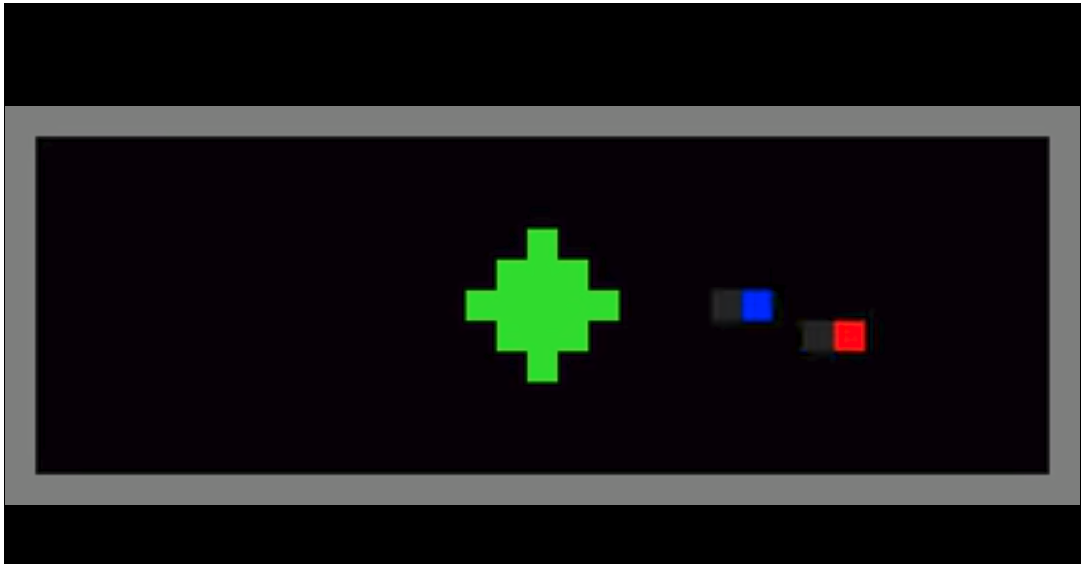
\includegraphics[width=1\textwidth]{figures/gath.png}
				\caption{Gathering Environment}
				\label{fig:Gather}
			\end{subfigure}
			\begin{subfigure}[b]{0.25\textwidth}
				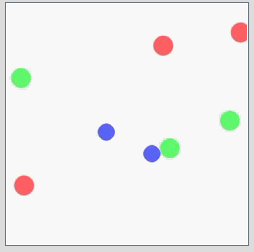
\includegraphics[width=1\textwidth]{figures/water.png}
				\caption{Waterworld Environment}
				\label{fig:water}
			\end{subfigure}
			\caption{Multi-Agent Environments}
			\label{fig:environments}
\end{figure}
		
Being inspired by multi-agent RL (MARL) problems\cite{Buşoniu2008} in robotics and resource management, we want to start with an actor-critic algorithm which adopts an idea of using centralized critic decentralized actor. There are several implementations of that method, for instance, Multi-Agent Deep Deterministic Policy Gradients (MADDPG) algorithm proposed in Lowe's paper \cite{lowe2017} utilizing individual DDPG policy networks for actor and shared Q-value network for critic. Artificial agents trained by deep multi-agent reinforcement learning to study the complex sequential social dilemmas have demonstrated feasibility of solution in complex virtual environments like Waterworld \cite{pytorch} shown in Fig. \ref{fig:environments}\subref{fig:water} and Gathering game shown in Fig \ref{fig:environments}\subref{fig:Gather} where two agents share world and collect apples to receive positive rewards\cite{deepmind}. We are going to start with a simplified environment like LunarLander modified for MARL purpose.
		
\section{Environment}
To minimize the effort of tuning other environments, we modified the environment that we used in one of the homeworks called LunarLander. LunarLander is a original OpenAI GYM environment built using Box2D package \cite{1606.01540}. In that environment, the agent can control a lander with a choice of discrete or continuous action sets. In discrete set, there are 4 actions - left and right engine's thrust and main engine thrust pointing down. In continuous version, the control is provided by a 2-dimensional vector controlling left/right thrust independently from main engine thrust. The observation space is given by the tuple of various parameters shown in Eq. \ref{eq:orig_state}.
The reward system in the original environment given by continuous reward given by squared distance to landing zone and error in additional state parameters such as vector velocity, angular orientation and velocity, and discrete additional reward for successful landing or penalty for leaving the screen or crash as demonstrated in Eq. \ref{eq:orig_rew}.
\begin{align}
\text{State} = [X_\text{err},Y_\text{err}, V_{x}, V_{y}, A_\text{rot},W_\text{rot},C_\text{leg1},C_\text{leg2}]
\label{eq:orig_state}
\end{align}
\begin{align}
\text{Reward} = &X^2_\text{err} + Y^2_\text{err} + V^2_{x} + V^2_{y} + A^2_\text{rot} + W^2_\text{rot} + \text{R}_\text{step}
\label{eq:orig_rew}\\
\text{R}_\text{step} = &+100\text{ if landed}\\
&-100\text{ if crashed or left}
\end{align}

To fit our needs, we modified the existing environment by adding the second lander that can be controlled independently. Both landers works completely parallel without collisions sharing state space and the landing zone. The only interaction between landers occurs in a new reward system that mixes rewards of both landers into one. That makes the problem very complex since the agents don't really understand if the change in the reward is made by themselves or the opponents.

\begin{align}
\text{State} = [[X_\text{err},Y_\text{err}, V_{x}, V_{y}, A_\text{rot},W_\text{rot},C_\text{leg1},C_\text{leg2}]_\text{lander1},\\
[X_\text{err},Y_\text{err}, V_{x}, V_{y}, A_\text{rot},W_\text{rot},C_\text{leg1},C_\text{leg2}]_\text{lander2}] 
\end{align}
\begin{align}
\text{Reward} = &R_\text{lander1} + R_\text{lander2} + R_\text{step} \textit{ if } (R_\text{lander1} R_\text{lander2}) \ge 0
\label{eq:new_rew}\\
&R_\text{step} \textit{ else} \\
R_\text{step} = &+100\textit{ if } \text{both landed}\\
&-100\textit{ if } \text{both crashed or left}
\end{align}

The reward system has been modified several times during the main set of experiments in order to maximize the effect of training. We found that sum of rewards from two lander as shown in Eq. \ref{eq:new_rew} may positively reinforce the wrong behavior explored by the agents that affects the whole training progress. To resolve the issue, we came up with an idea of providing the reward only when both agents doing well or both doing bad. In this case, it allows to reinforce the policy using a proper gradient of payoff and avoid the misleading reinforcement.

\section{Models}

Our model is based on GA3C by Babaeizadeh {\it et. al.}\cite{babaeizadeh2016} (hybrid version of Asynchronous Advantage Actor-critic algorithm)\footnote{Original code can be found at \href{https://github.com/NVlabs/GA3C}{https://github.com/NVlabs/GA3C}} and adopts the idea of multi-agent decentralized actor, centralized critic approach where the critic is augmented with extra information about the policies of other agents, while the actor only has access
to local information\cite{lowe2017}.

The policy gradient for each agent is described in Eq. \ref{grad}: Each agent has its own policy $\pi_i(a_{t, i}|s_t, \theta)$ with regard of its own action $a_{t, i}$ and current state $s_t$ but the advantage function $A(s_t, a_{t, 1}, ..., a_{t, N}$ is shared by all agents. The advantage function is estimated by the temporal difference function $\delta_t$ (Eq. \ref{advantage}).
\begin{equation}
\nabla_{\theta}\eta_i(\pi_{\theta}) = E_{\tau}[\sum^{T-1}_{t=0}\nabla_{\theta}\log\pi_i(a_{t, i}|s_t, \theta)A(s_t, a_{t, 1}, ..., a_{t, N}) + \beta\sum^{T-1}_{t=0}\nabla_{\theta}H(s_t|\theta)]
\label{grad}
\end{equation}
\begin{equation}
\hat{A}(s_t, a_{t, 1}, ..., a_{t, N}) = \sum^{\infty}_{t=0} (\gamma \lambda)^l \delta_{t+l}
\label{advantage}
\end{equation}

Because our LunarLander environment is continuous, the policy for each agent is chosen to be Gaussian distribution as shown in Eq. \ref{poli}. Action mean $\mu_{\theta}(s_t)$ is a two hidden layers feedforward neural network of which output is 2-dimensional and standard deviation $\sigma$ is given.
\begin{align}
\pi_i(a_{t, i}|s_t) = & \frac{1}{\sqrt{2\pi} \sigma_{1, i}} \exp( -\frac{(a_{t, i}^{(1)}-\mu_{\theta, i}(s_t)^{(1)})^2}{2\sigma_{1, i}^2}) \nonumber \\
& \cdot \frac{1}{\sqrt{2\pi} \sigma_{2, i}} \exp( -\frac{(a_{t, i}^{(2)}-\mu_{\theta, i}(s_t)^{(2)})^2}{2\sigma_{2, i}^2})
\label{poli}
\end{align}

In addition to the policy gradient, we also trained the critic function using linear regression where the value is also a two hidden layers feedforward neural network of which output is a single value. By default, the number of hidden units of value network are twice of that in action mean network.

\section{Results}

As mentioned before, in order to compute the action mean network, we tried two strategies: (a) using 2 independent network for each agent's action mean with same state as input (so-called 2 actor) or (b) using the same network for both action means but each agent has different state input (so-called 1 actor). We expected to see similar performance between these two strategies because the two agents should have very similar policy when trained successfully; however, in contrast to what we thought, the single network for action mean (1 actor) doesn't perform well due to its simplicity (see yellow and purple curves in Fig. \ref{fig:actor_reward}). The purple curve completely failed to train while the yellow curve also diverged at the end of train.

\begin{figure}[htbp]
	\centering
	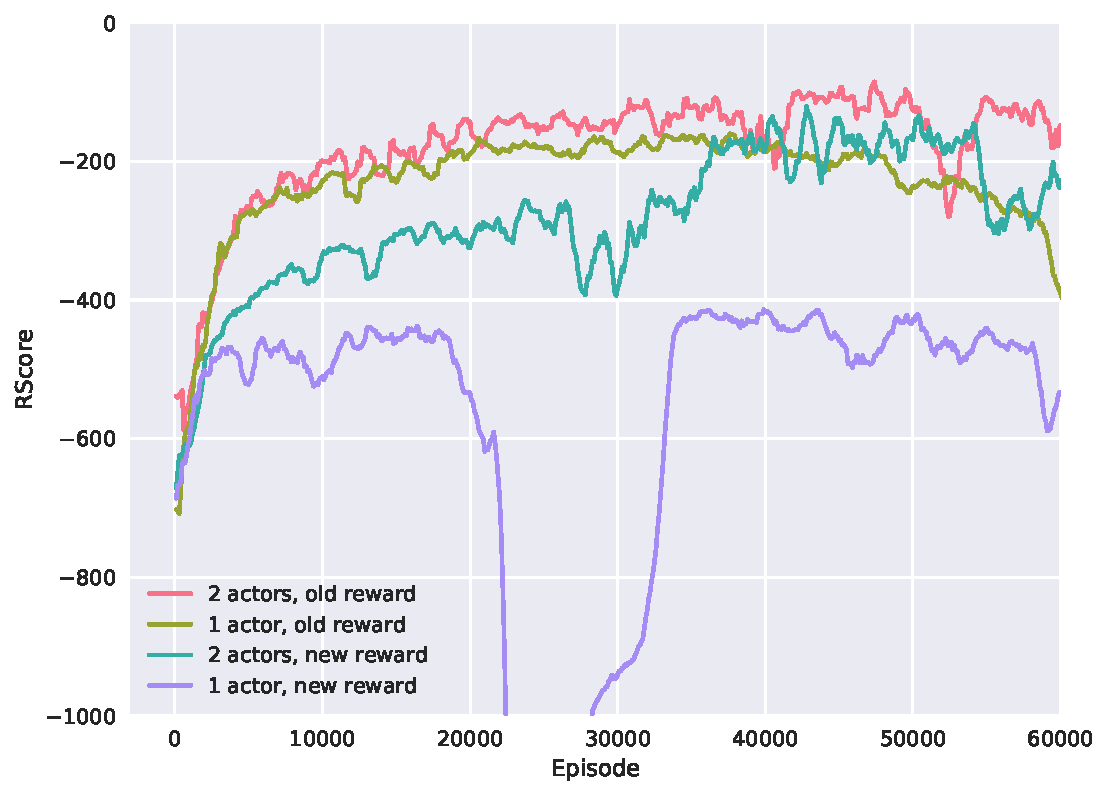
\includegraphics[width=0.8\textwidth]{figures/actor_reward_comparison.pdf}
	\caption{Learning curves with different actors and reward system}
	\label{fig:actor_reward}
\end{figure}

The old reward system has a higher payout than the new one therefore it reaching a similar score as with the new reward system actually means the old reward system was stuck in some local minimum where one of the agent quickly falls down to the target landing zone while the other one keeps hovering around in the air (Fig \ref{fig:fail}). The Fig. \ref{fig:actor_reward} shows the best model (blue curve) is using 2 independent network for each action mean with the new reward system.

\begin{figure}[htbp]
	\centering
	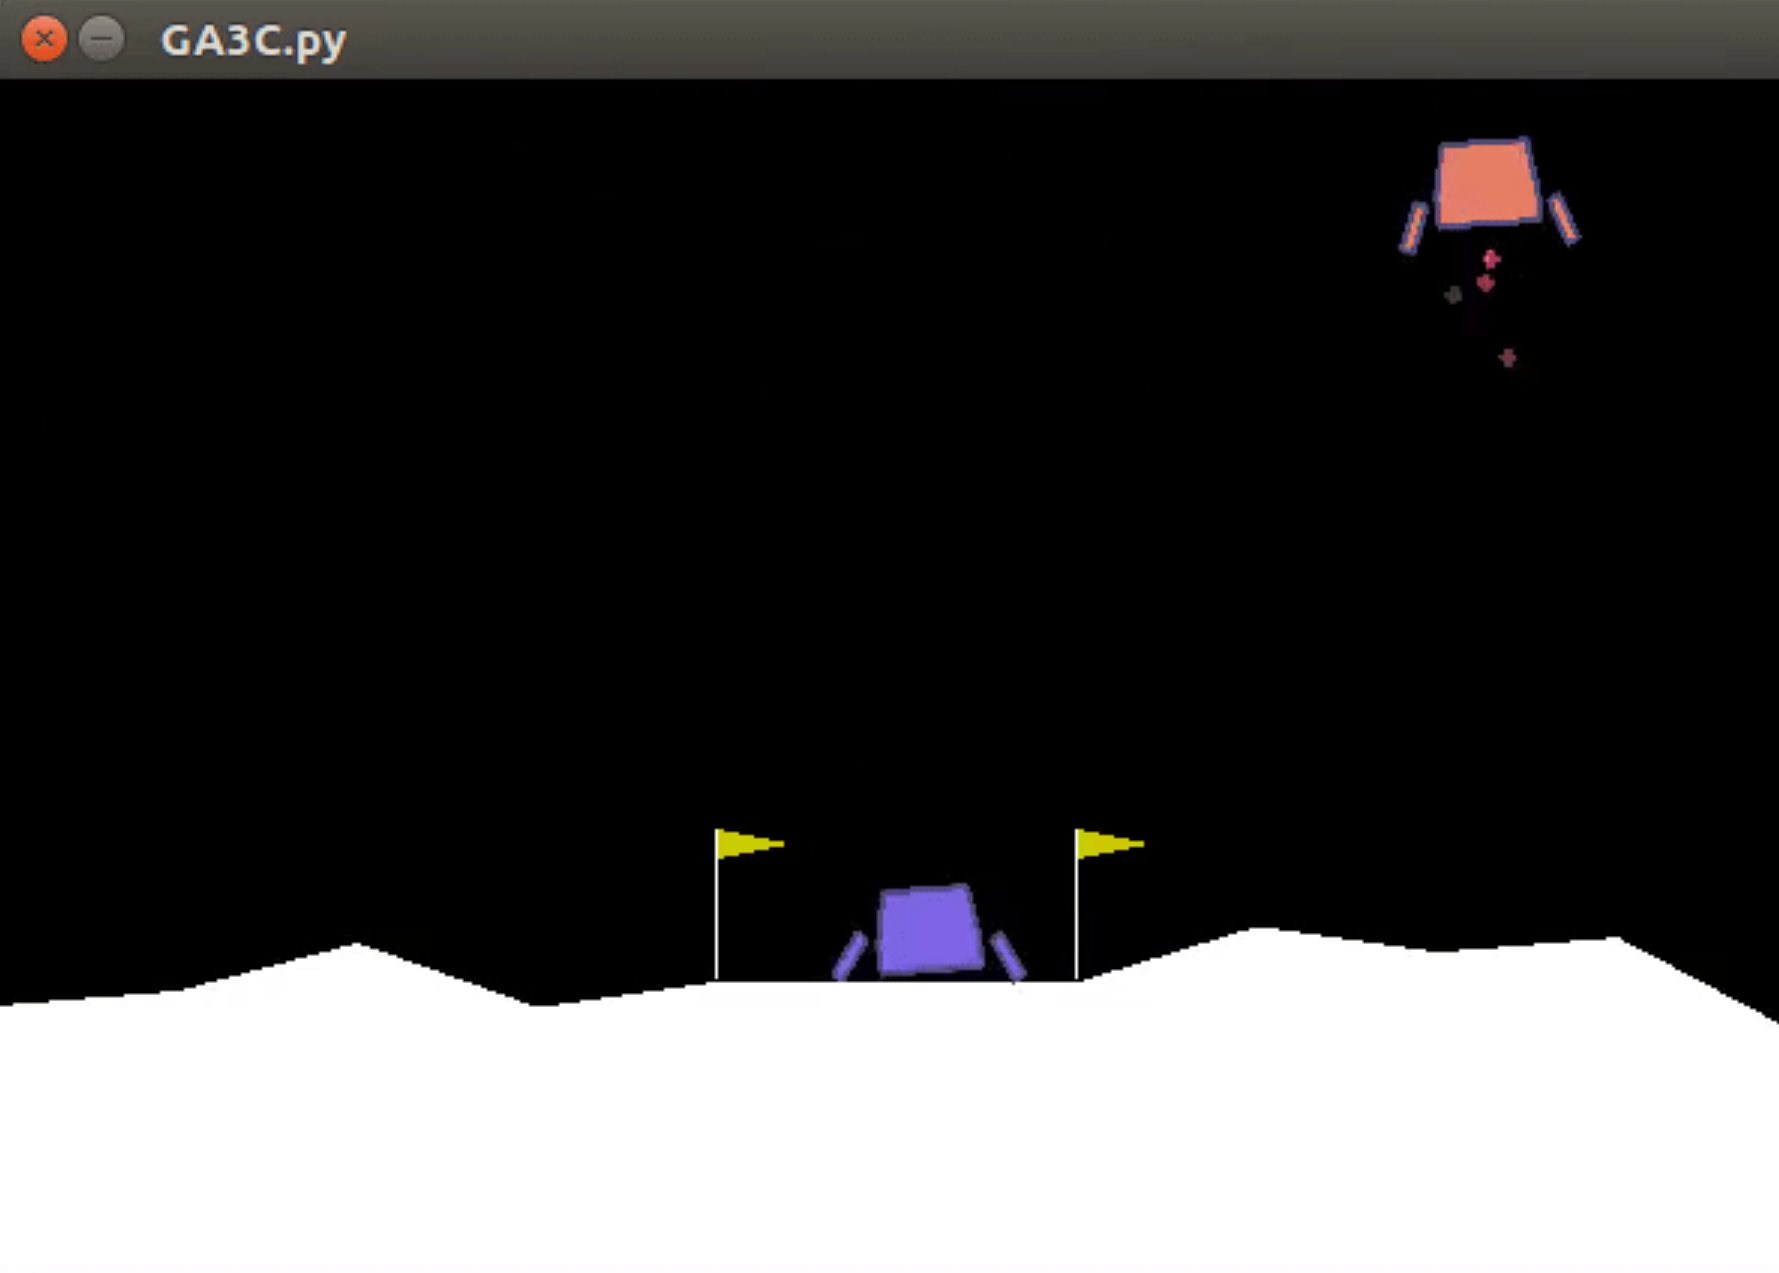
\includegraphics[width=0.8\textwidth]{figures/fail.png}
	\caption{Failed policy with old reward system}
	\label{fig:fail}
\end{figure}

In order to tune the hyper-parameters, we tested $\lambda$ and $\beta$ which is bias-variance trade-off and regularization factor respectively (Fig. \ref{fig:params}). Unlike the single agent problem, the $\lambda$ plays a more important role than $\beta$ such that the model failed to train when $\lambda$ is slightly away from 1. The best $\lambda$ value agrees with our approximation of the advantage function: when $\lambda=1$ the advantage function takes all future rewards into consideration and yields much lower bias (Eq. \ref{advantage2}).
\begin{equation}
\hat{A}(s_t, a_t) = \sum^{\infty}_{t=0} \gamma^l r_{t+l} - V(s_t)
\label{advantage2}
\end{equation}

\begin{figure}[htbp]
	\centering
	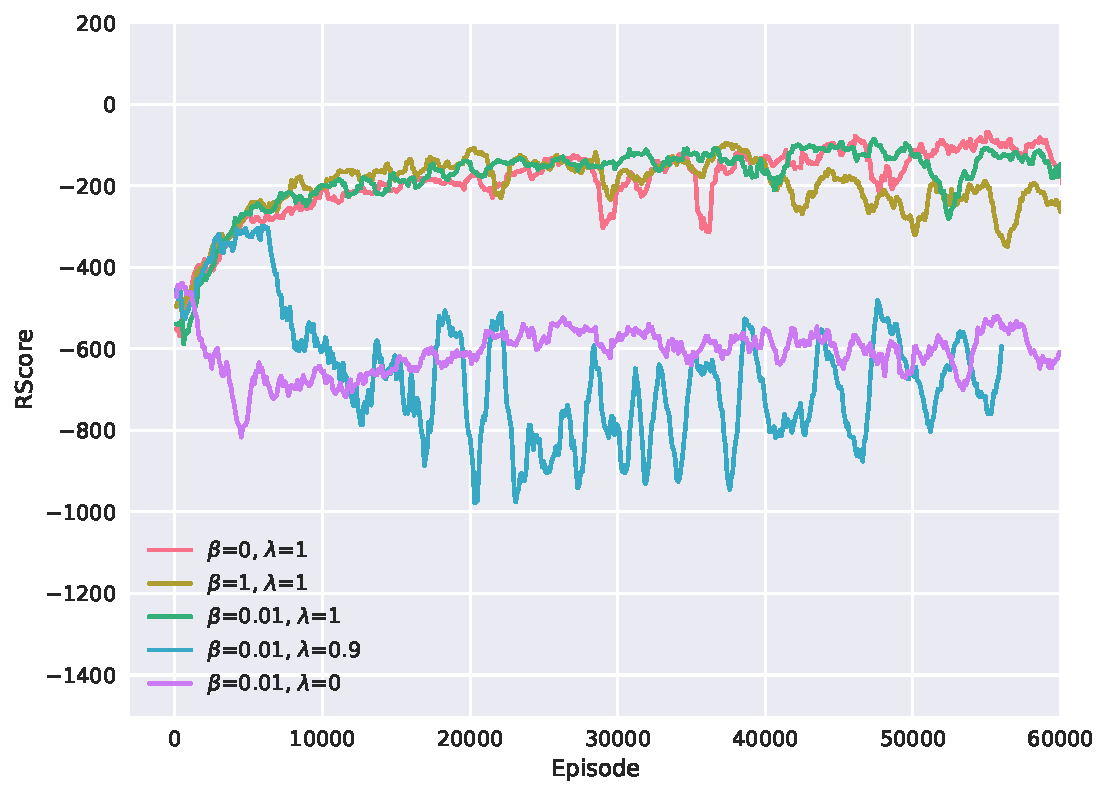
\includegraphics[width=0.8\textwidth]{figures/lambda_beta_comparison.pdf}
	\caption{Learning curves with different $\lambda$ and $\beta$}
	\label{fig:params}
\end{figure}

We also tested the impacts of number of hidden units in action mean network (the number of hidden units in value network is simultaneously twice of that in value network) as shown in Fig. \ref{fig:units}. The optimal number is 64 among the three numbers we tried.

\begin{figure}[htbp]
	\centering
	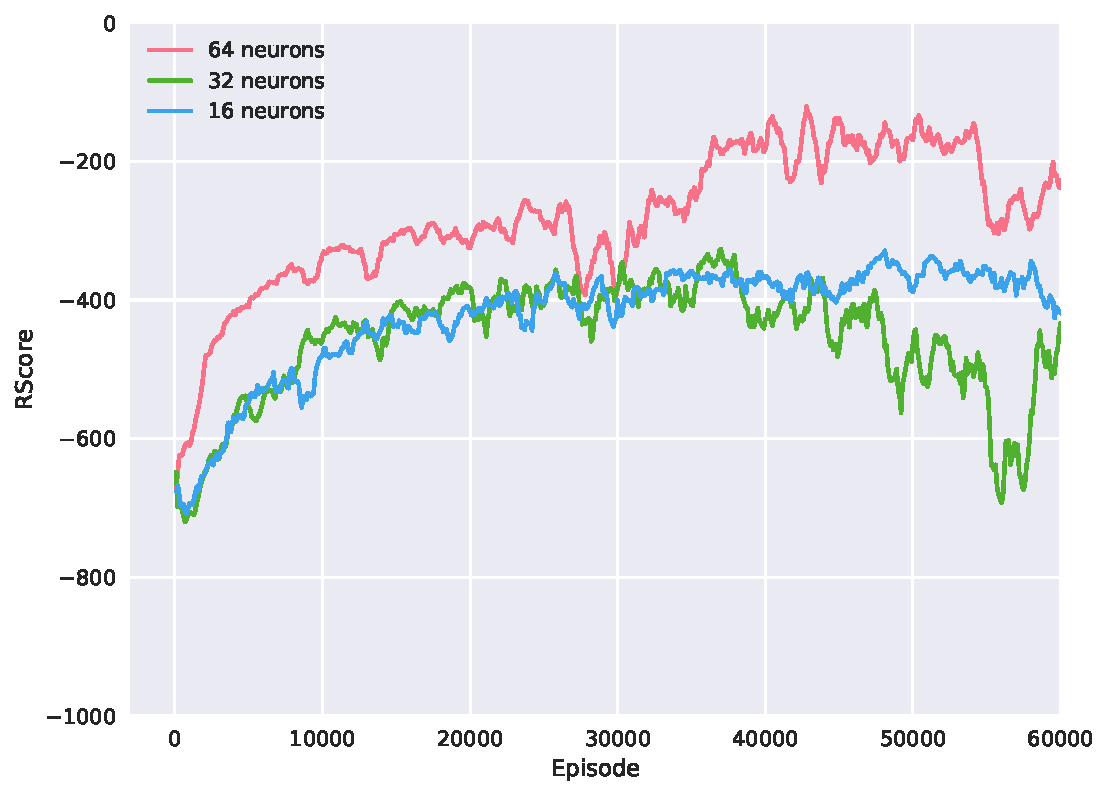
\includegraphics[width=0.8\textwidth]{figures/neurons_comparison.pdf}
	\caption{Learning curves with different number of hidden units in action mean network}
	\label{fig:units}
\end{figure}

Finally, our best model of two agents with all tuned hyper-parameters is shown in Fig. \ref{fig:success}.

\begin{figure}[htbp]
	\centering
	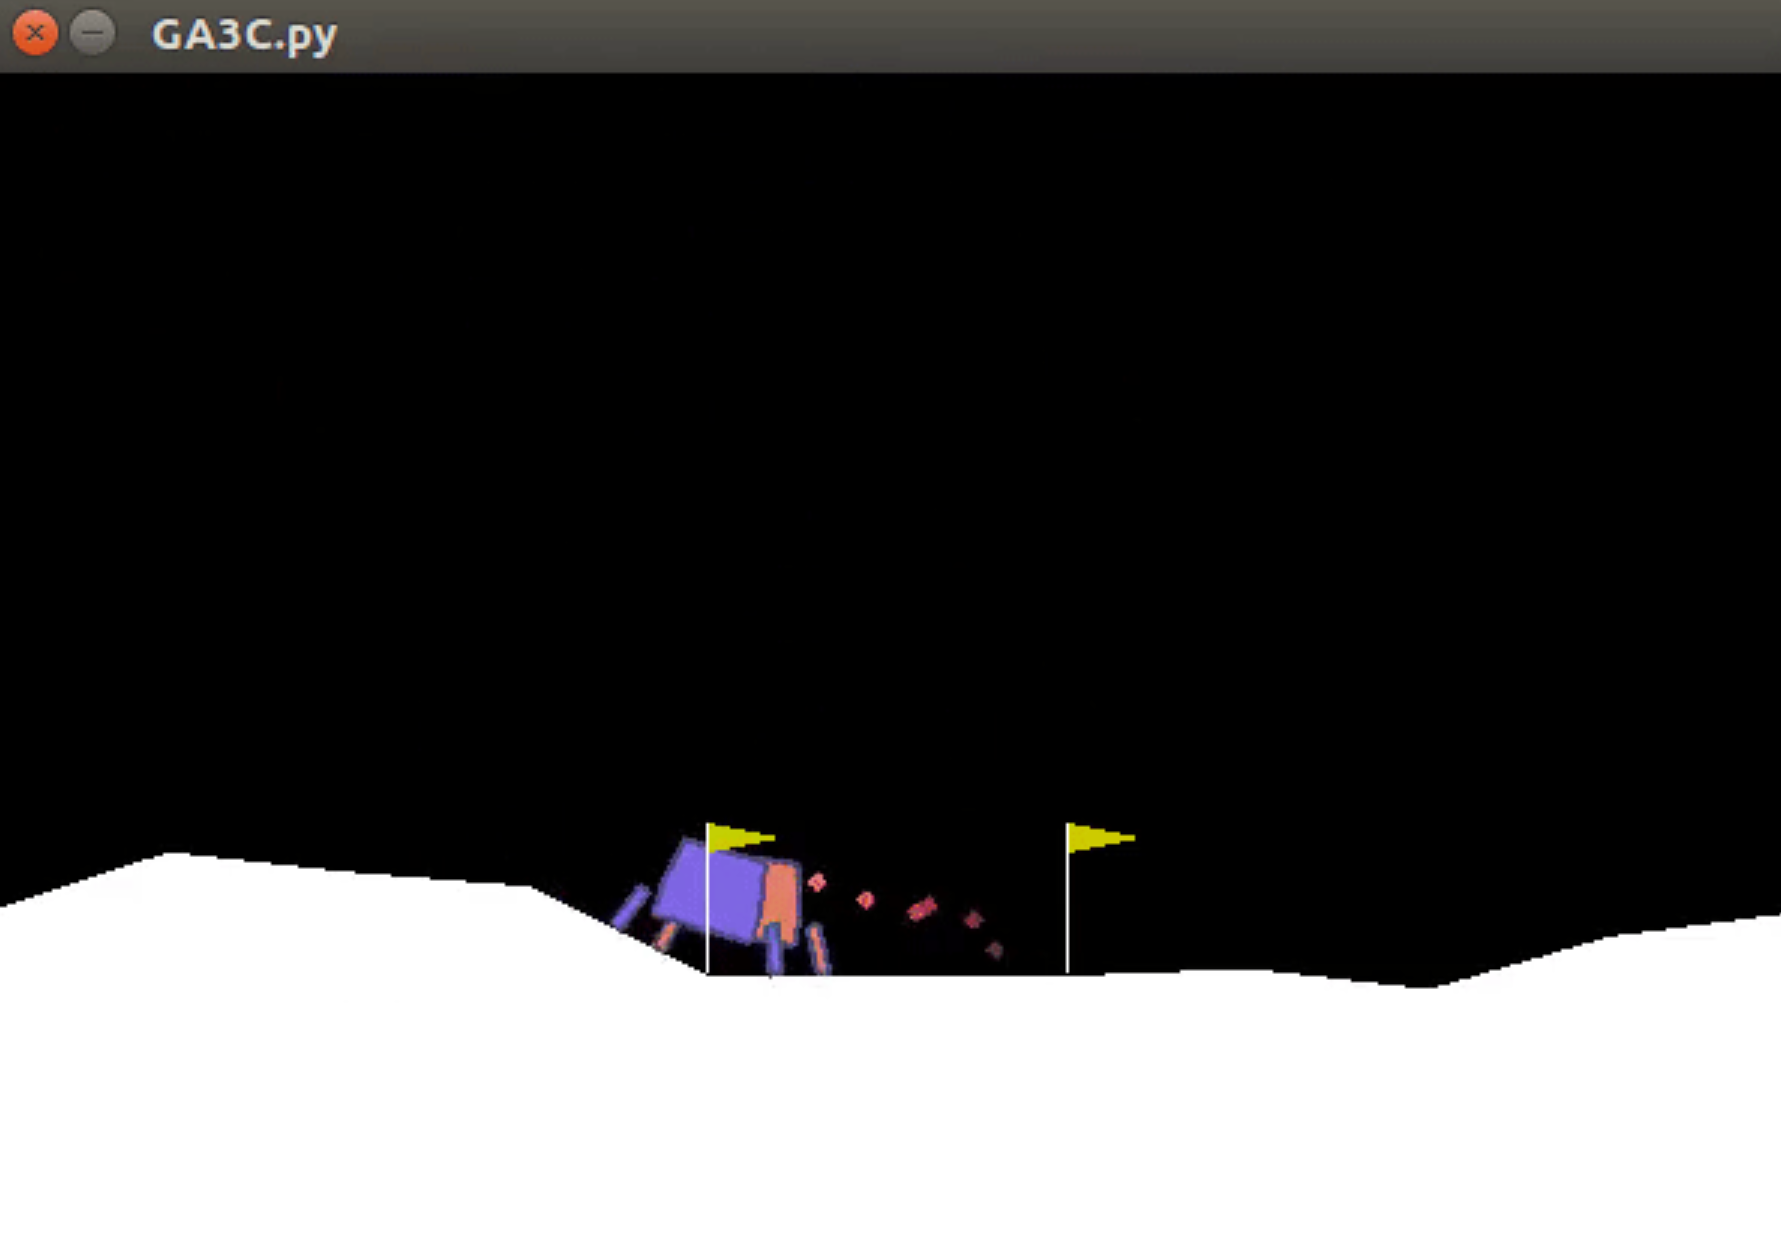
\includegraphics[width=0.8\textwidth]{figures/success.png}
	\caption{Final successful policy best model and tuned parameters}
	\label{fig:success}
\end{figure}

\section{Conclusion}
In this project, we demonstrated that the complex MARL task may be solved using the shared critic approach. The choice of the algorithms for actor is not limited to DDPG algorithm demonstrated in the literature, but any policy based network would provide a feasible solution. This work demonstrates hyper-parameters that achieved the best rate of convergence for our problem.
Local policy actor with shared critic is a possible solution for MARL type of problems that are very complex problems due to noisy and unstable solutions. This result fits the similar difficulties discussed in the original paper experiencing noisy transitions that caused high variance in solutions.

Success of training is impossible without careful reward system planning. Adding more agents causing additional very strong sub optimal policies that attracts the algorithm to converge to the wrong policy. Therefore, each task requires careful thinking of the reward and stopping criteria to allows the convergence. However, those changes are environment specific and cannot be easily extended to other environments. Each task requires much fine tuning and not transferable from problem to problem.


\newpage
\bibliographystyle{abbrv}
\bibliography{ref}

\end{document}